\documentclass{scrreprt}

\usepackage[english,ngerman]{babel} 
\usepackage[utf8]{inputenc} 
\usepackage{graphicx}
\usepackage{dsfont}
\usepackage{amsmath}

\title{TH1 - Aufgabenblatt 2}
\author{Andreas Krohn, Erik Andresen, Benjamin Vetter, Andreas Basener}

\begin{document}

\maketitle

\begin{enumerate}

\item Welche Eigenschaften sollte Eure Gleisanlage haben? (informelle Beschreibung)

\begin{itemize}
  \item Deadlock-Freiheit
  \item Starvation-Frei
  \item Beschränkt bzgl. der maximalen Anzahl an fahrenden Zügen pro Gleisabschnitt
  \item Kollisionsfrei
  \item Alpenpanorama
\end{itemize}

\newpage

\item Modellierung:

(a) Modelliert die einzelnen o.g. Gleise, Weichen und die Schranke jeweils mit
    einem eigenen S/T-Netz. Wie werden die Züge darin modelliert?


Ein Gleis ist eine Stelle mit maximaler Belegung von eins. Wenn ein Zug dieses Gleis belegt befindet sich auf der Stelle ein Token.
Die Weichen werden über zwei alternative Transitionen, die von der Stelle weglaufen modelliert: Pro Weiche und Richtung existiert eine Transition, d.h. über das Schalten der
jeweiligen Transition wird gewählt wie der Zug weiterfahren soll.

Der Bahnübergang ist eine Transition auf der Bahnstrecke zwischen zwei Gleisabschnitten (Stellen), die nur schaltet wenn sich niemand auf dem Bahnübergang befindet (Token auf Bahnübergang frei). Wird der Bahnübergang (Bü) betreten befindet sich kein Token mehr auf "`Bahnübergang frei"' und damit kann der Zug den Bahnübergang nicht passieren.
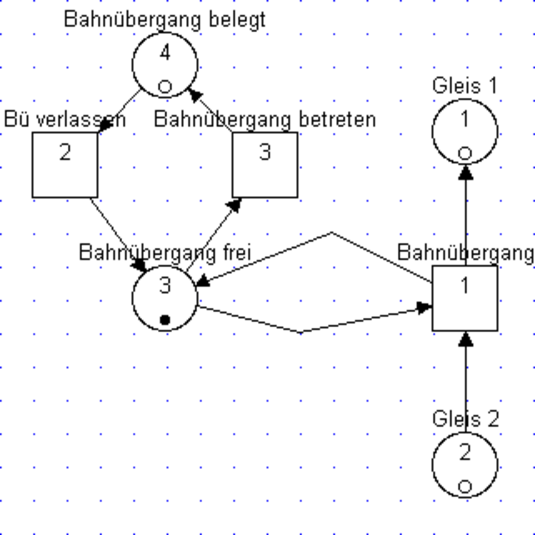
\includegraphics[width=0.45\textwidth]{bahnuebergang.pdf}

(b) Setzt die einzelnen S/T-Netze zusammen, so dass mind. jedes Gleis, jede Weiche und die Schranke einmal in Eurer Gleisanlage vorhanden sind und gebt eine Anfangsmarkierung mit zwei Zügen an.
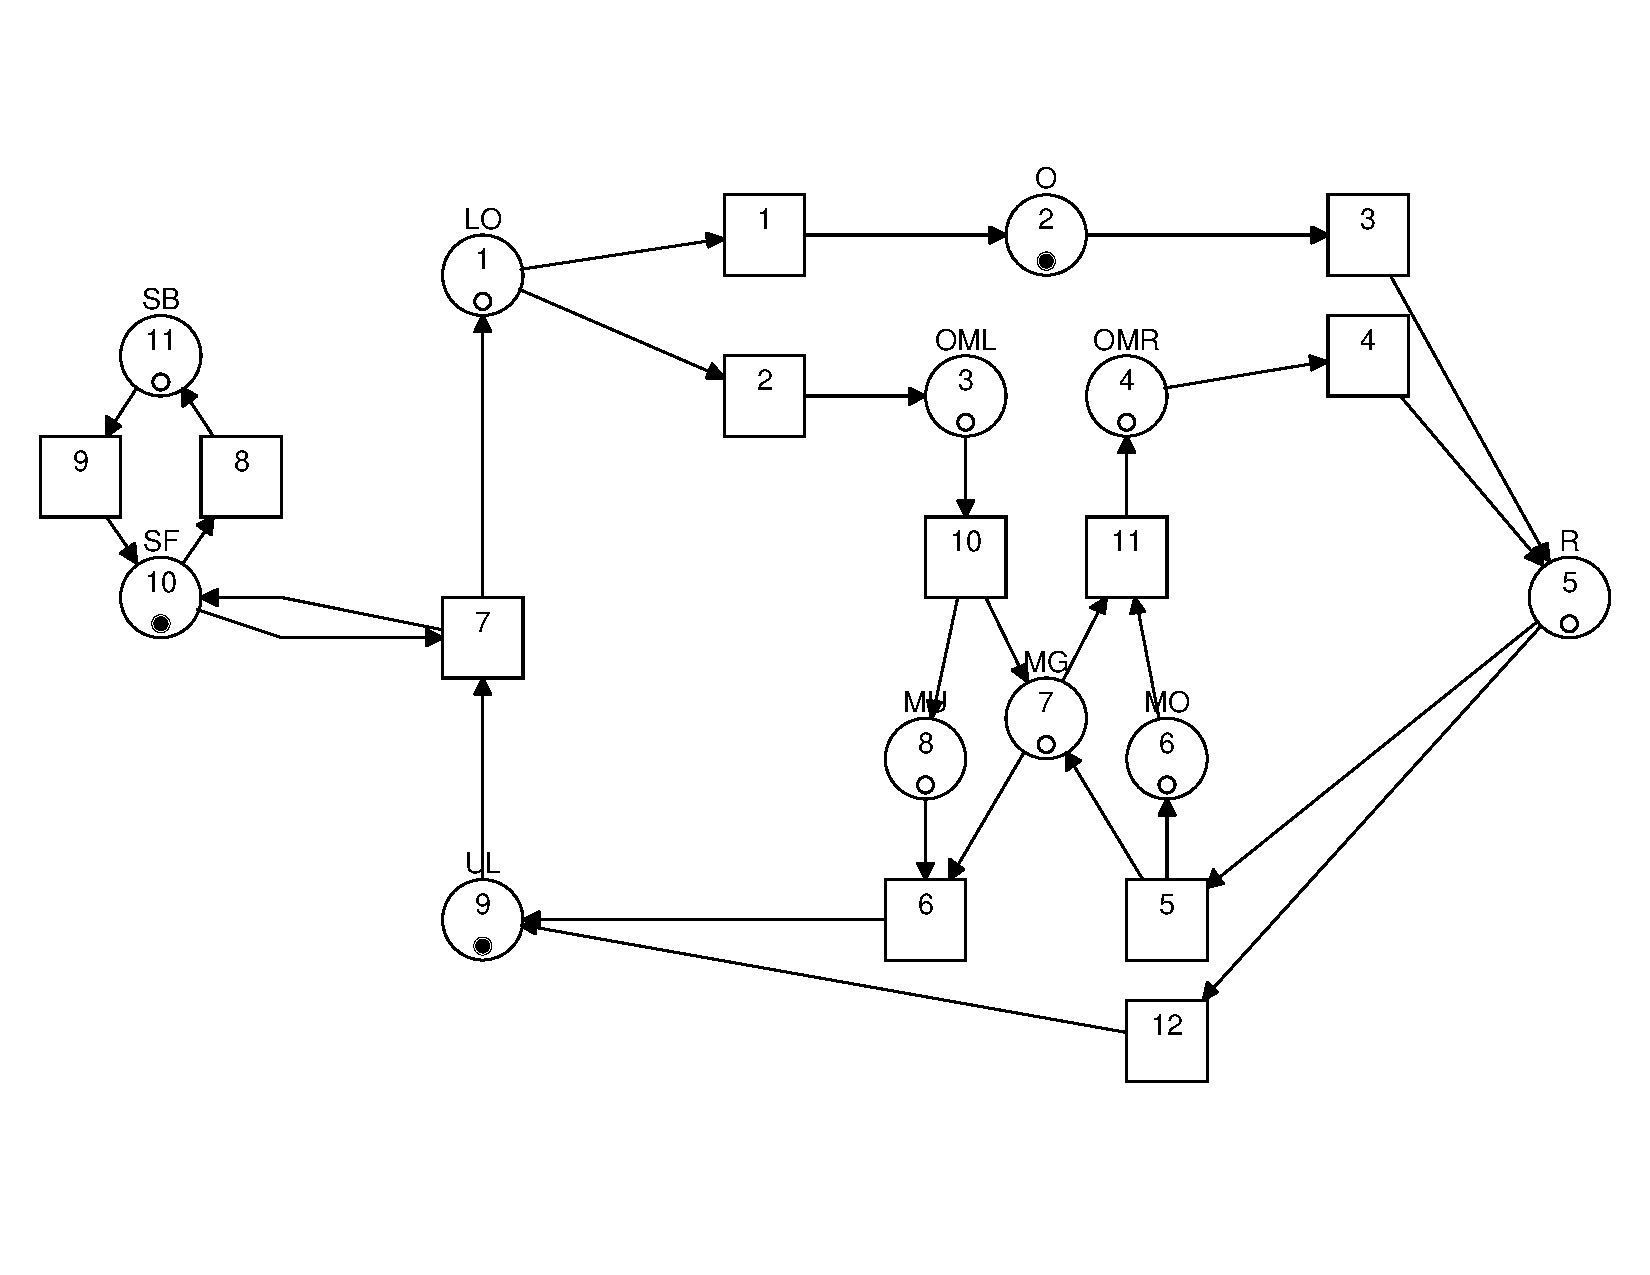
\includegraphics[width=1\textwidth]{prak2_aufg2.pdf}

\item Analyse:

(a) Berechnet die P-Invarianten Euer Gleisanlage.
(b) Berechnet die T-Invarianten Euer Gleisanlage.
(c) Berechnet den Erreichbarkeitsgraph Eurer Gleisanlage.
(d) Berechnet den Kondensationsgraph Eurer Gleisanlage.
(e) Berechnet den Uberdeckungssgraph Eurer Gleisanlage.


\end{enumerate}

\end{document}

% vim: fileencoding=utf8
